\documentclass[aspectratio=169,11pt]{beamer}
\usetheme{default}
\usecolortheme{default}

\setbeamertemplate{navigation symbols}{}
\setbeamertemplate{footline}[frame number]

\usepackage{amsmath}
\usepackage{booktabs}
\usepackage{graphicx}
\usepackage{tikz}
\usetikzlibrary{arrows.meta, calc, patterns, positioning, shapes.geometric}

\newcommand{\etal}{et al.}

\title{The Micro-Scale Picture Inside a Macro-Scale Porous Reactor}
\subtitle{How pore-scale BZ reaction--diffusion dynamics scale up}
\author{Srivijayesh Venugopal}
\date{Cranfield IRP 2025-26}

\begin{document}

\begin{frame}
\titlepage
\end{frame}

% ---------------------------------------------------------------------
\begin{frame}{The macro-scale reactor: a porous medium filled with BZ chemistry}

\begin{columns}[T]
\begin{column}{0.55\textwidth}
\centering
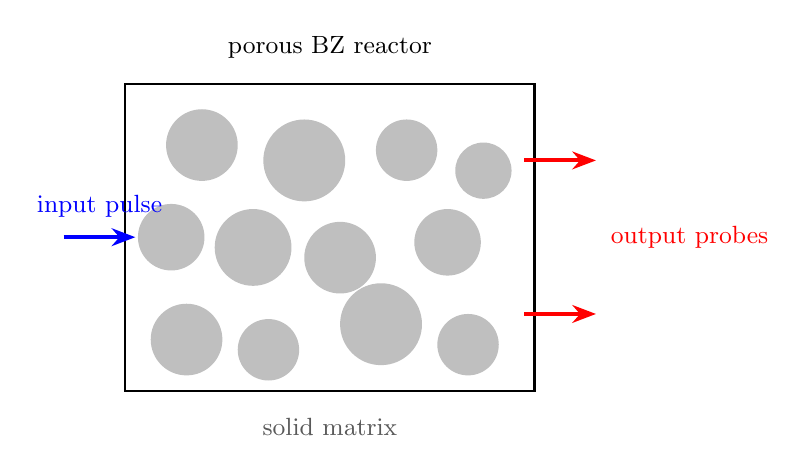
\begin{tikzpicture}[scale=0.65, every node/.style={font=\small}]
  % outer boundary
  \draw[thick] (0,0) rectangle (8,6);
  % solid grains
  \foreach \x/\y/\r in {1.2/1.0/0.7, 2.8/0.8/0.6, 5.0/1.3/0.8, 6.7/0.9/0.6,
                          0.9/3.0/0.65, 2.5/2.8/0.75, 4.2/2.6/0.7, 6.3/2.9/0.65,
                          1.5/4.8/0.7, 3.5/4.5/0.8, 5.5/4.7/0.6, 7.0/4.3/0.55}
    \fill[gray!50] (\x,\y) circle (\r);
  % input arrow
  \draw[-{Stealth[length=3mm]}, line width=1.5pt, blue] (-1.2,3) -- (0.2,3);
  \node[blue, above] at (-0.5,3.2) {input pulse};
  % output arrows
  \draw[-{Stealth[length=3mm]}, line width=1.5pt, red] (7.8,1.5) -- (9.2,1.5);
  \draw[-{Stealth[length=3mm]}, line width=1.5pt, red] (7.8,4.5) -- (9.2,4.5);
  \node[red, right] at (9.3,3) {output probes};
  % labels
  \node[gray!70!black] at (4,-0.7) {solid matrix};
  \node at (4,6.7) {porous BZ reactor};
\end{tikzpicture}
\end{column}
\begin{column}{0.42\textwidth}
\textbf{What you see at the lab scale:}
\begin{itemize}
    \item A slab of porous material (gel, membrane, 3D-printed scaffold) saturated with Belousov--Zhabotinsky reagents.
    \item Input: a chemical or light stimulus at one face.
    \item Output: optical readout of oxidised-catalyst concentration at another face.
    \item The internal geometry is too fine to resolve easily.
\end{itemize}
\end{column}
\end{columns}

\vspace{0.4cm}
\textbf{Question:} What is actually happening inside the pores?

\end{frame}

% ---------------------------------------------------------------------
\begin{frame}{Zoom in: the pore network is a graph of throats and junctions}

\begin{columns}[T]
\begin{column}{0.55\textwidth}
\centering
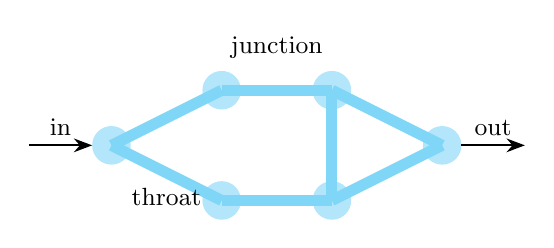
\begin{tikzpicture}[scale=0.7, every node/.style={font=\small}]
  % pores as nodes
  \foreach \x/\y/\n in {1/3/A, 3/4/B, 3/2/C, 5/4/D, 5/2/E, 7/3/F}
    \fill[cyan!30] (\x,\y) circle (0.35) node {\n};
  % throats as edges
  \draw[line width=4pt, cyan!50] (1,3) -- (3,4);
  \draw[line width=4pt, cyan!50] (1,3) -- (3,2);
  \draw[line width=4pt, cyan!50] (3,4) -- (5,4);
  \draw[line width=4pt, cyan!50] (3,2) -- (5,2);
  \draw[line width=4pt, cyan!50] (5,4) -- (5,2);
  \draw[line width=4pt, cyan!50] (5,4) -- (7,3);
  \draw[line width=4pt, cyan!50] (5,2) -- (7,3);
  % labels
  \node[below] at (2,2.4) {throat};
  \node[above] at (4,4.4) {junction};
  \draw[-{Stealth}, thick] (-0.5,3) -- (0.65,3) node[midway, above] {in};
  \draw[-{Stealth}, thick] (7.35,3) -- (8.5,3) node[midway, above] {out};
\end{tikzpicture}
\end{column}
\begin{column}{0.42\textwidth}
\textbf{The pore network is a graph:}
\begin{itemize}
    \item \textbf{Pores} = bulbous voids where fluid can accumulate.
    \item \textbf{Throats} = narrow connections between pores.
    \item \textbf{Junctions} = places where multiple throats meet.
\end{itemize}

\vspace{0.3cm}
\textbf{Information carrier:} a pulse of oxidised catalyst (the ``blue'' wave in BZ) travelling through the pore fluid.

\end{column}
\end{columns}

\vspace{0.4cm}
\textbf{Key insight:} each element of this graph has a direct analogue in our structured 2D simulations.

\end{frame}

% ---------------------------------------------------------------------
\begin{frame}{Pore throat = straight channel (the wire)}

\begin{columns}[T]
\begin{column}{0.48\textwidth}
\centering
\textbf{Pore throat (3D view)}\\[0.3cm]
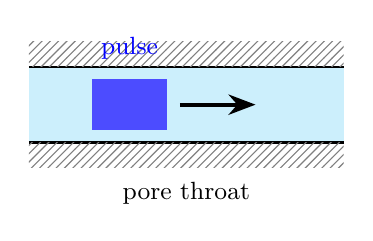
\begin{tikzpicture}[scale=0.8, every node/.style={font=\small}]
  % throat as a tube
  \fill[cyan!20] (0,-0.6) rectangle (5,0.6);
  \draw[thick] (0,-0.6) -- (5,-0.6);
  \draw[thick] (0,0.6) -- (5,0.6);
  % walls
  \fill[pattern=north east lines, pattern color=gray] (0,0.6) rectangle (5,1.0);
  \fill[pattern=north east lines, pattern color=gray] (0,-1.0) rectangle (5,-0.6);
  % pulse
  \fill[blue!70] (1,-0.4) rectangle (2.2,0.4);
  \draw[-{Stealth}, line width=1.5pt] (2.4,0) -- (3.6,0);
  % labels
  \node at (2.5,-1.4) {pore throat};
  \node[blue] at (1.6,0.9) {pulse};
\end{tikzpicture}
\end{column}
\begin{column}{0.48\textwidth}
\centering
\textbf{Our 2D model}\\[0.3cm]
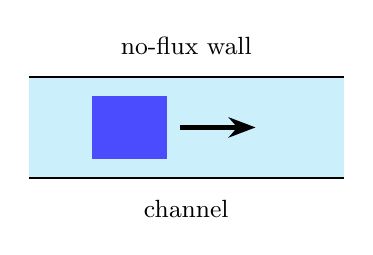
\begin{tikzpicture}[scale=0.8, every node/.style={font=\small}]
  % channel
  \fill[cyan!20] (0,-0.8) rectangle (5,0.8);
  \draw[thick] (0,-0.8) -- (5,-0.8);
  \draw[thick] (0,0.8) -- (5,0.8);
  % pulse
  \fill[blue!70] (1,-0.5) rectangle (2.2,0.5);
  \draw[-{Stealth}, line width=1.5pt] (2.4,0) -- (3.6,0);
  % labels
  \node at (2.5,-1.3) {channel};
  \node at (2.5,1.3) {no-flux wall};
\end{tikzpicture}
\end{column}
\end{columns}

\vspace{0.5cm}
\textbf{What the transfer function tells us:}
\begin{itemize}
    \item The pulse speed is set by the kinetics, not by the throat width.
    \item A straight throat is a near-perfect wire: 6.46 cells/t.u., no width-induced block down to one cell.
    \item In 3D, the same behaviour holds: measured speed 6.62 cells/t.u.
\end{itemize}

\end{frame}

% ---------------------------------------------------------------------
\begin{frame}{Pore junction = T-junction (the switch)}

\begin{columns}[T]
\begin{column}{0.48\textwidth}
\centering
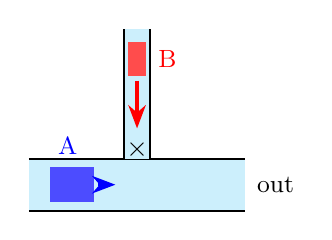
\begin{tikzpicture}[scale=0.55, every node/.style={font=\small}]
  % horizontal channel
  \fill[cyan!20] (0,-0.6) rectangle (5,0.6);
  \draw[thick] (0,-0.6) -- (5,-0.6);
  \draw[thick] (0,0.6) -- (5,0.6);
  % vertical channel
  \fill[cyan!20] (2.2,0.6) rectangle (2.8,3.6);
  \draw[thick] (2.2,0.6) -- (2.2,3.6);
  \draw[thick] (2.8,0.6) -- (2.8,3.6);
  % pulses
  \fill[blue!70] (0.5,-0.4) rectangle (1.5,0.4);
  \fill[red!70] (2.3,2.5) rectangle (2.7,3.3);
  % arrows
  \draw[-{Stealth}, line width=1.2pt, blue] (1.6,0) -- (2.0,0);
  \draw[-{Stealth}, line width=1.2pt, red] (2.5,2.4) -- (2.5,1.3);
  % collision mark
  \node[black, font=\bfseries] at (2.5,0.8) {$\times$};
  % labels
  \node[blue] at (0.9,0.9) {A};
  \node[red] at (3.2,2.9) {B};
  \node at (5.7,0) {out};
\end{tikzpicture}
\end{column}
\begin{column}{0.48\textwidth}
\textbf{What happens at a junction:}
\begin{itemize}
    \item Two pulses entering from different throats collide and annihilate.
    \item The output throat stays silent: \textbf{inhibition} (A passes unless B vetoes it).
\end{itemize}

\vspace{0.2cm}
\textbf{Measured behaviour:}
\begin{itemize}
    \item A alone: output peak $\approx 0.71$
    \item B alone or A+B: output $\approx 0.003$ (rest-state floor)
    \item Separation ratio: $232\times$
\end{itemize}

\vspace{0.2cm}
\textbf{Readout trick:} probe in a short window aligned to A's arrival; otherwise the junction looks like OR.
\end{column}
\end{columns}

\end{frame}

% ---------------------------------------------------------------------
\begin{frame}{Pore geometry is the trainable substrate}

\begin{columns}[T]
\begin{column}{0.55\textwidth}
\centering
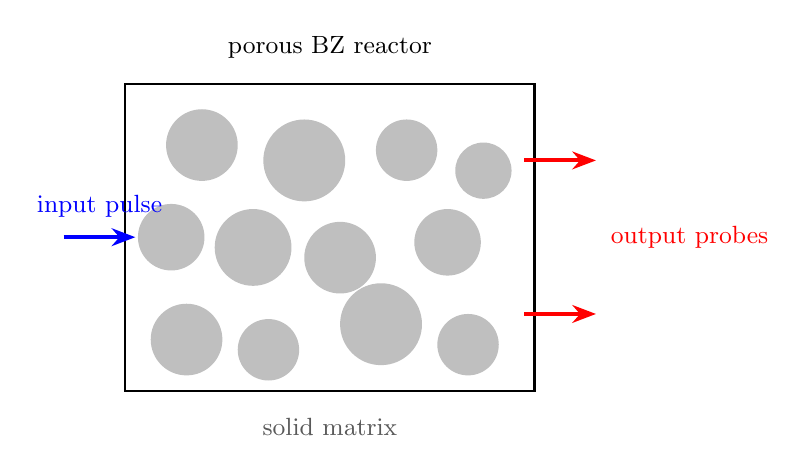
\begin{tikzpicture}[scale=0.65, every node/.style={font=\small}]
  % outer boundary
  \draw[thick] (0,0) rectangle (8,6);
  % solid grains
  \foreach \x/\y/\r in {1.2/1.0/0.7, 2.8/0.8/0.6, 5.0/1.3/0.8, 6.7/0.9/0.6,
                          0.9/3.0/0.65, 2.5/2.8/0.75, 4.2/2.6/0.7, 6.3/2.9/0.65,
                          1.5/4.8/0.7, 3.5/4.5/0.8, 5.5/4.7/0.6, 7.0/4.3/0.55}
    \fill[gray!50] (\x,\y) circle (\r);
  % input arrow
  \draw[-{Stealth[length=3mm]}, line width=1.5pt, blue] (-1.2,3) -- (0.2,3);
  \node[blue, above] at (-0.5,3.2) {input pulse};
  % output arrows
  \draw[-{Stealth[length=3mm]}, line width=1.5pt, red] (7.8,1.5) -- (9.2,1.5);
  \draw[-{Stealth[length=3mm]}, line width=1.5pt, red] (7.8,4.5) -- (9.2,4.5);
  \node[red, right] at (9.3,3) {output probes};
  % labels
  \node[gray!70!black] at (4,-0.7) {solid matrix};
  \node at (4,6.7) {porous BZ reactor};
\end{tikzpicture}
\end{column}
\begin{column}{0.42\textwidth}
\textbf{What the solid matrix controls:}
\begin{itemize}
    \item Pore size and throat width set pulse confinement.
    \item Junction topology sets collision and branching rules.
    \item Orientation of elongated pores sets anisotropic pulse delay.
    \item These are the ``weights'' of the macroscopic computation.
\end{itemize}

\vspace{0.3cm}
\textbf{2D analogue:} lithographed channels, 3D-printed scaffolds, or templated gels all impose the same geometry-driven constraints.
\end{column}
\end{columns}

\end{frame}

% ---------------------------------------------------------------------
\begin{frame}{The four pore-scale operators}

Every useful macroscopic behaviour must be built from these microscopic primitives:

\vspace{0.3cm}
\begin{table}
\centering
\footnotesize
\begin{tabular}{p{2.8cm}p{3.5cm}p{6.0cm}}
\toprule
\textbf{Operator} & \textbf{Pore-scale object} & \textbf{What it does} \\
\midrule
Wire & Straight throat & Transmits a pulse with fixed speed \\
Low-pass filter & Straight throat & Refractory tail drops fast pulse trains \\
Inhibition & Junction & Two colliding pulses annihilate \\
Delay / routing & Oriented pore structure & Anisotropy steers pulses without blocking \\
\bottomrule
\end{tabular}
\end{table}

\vspace{0.3cm}
\textbf{The ``instruction set'' is small.} A macroscopic porous reactor computes by combining these four operators in space.

\end{frame}

% ---------------------------------------------------------------------
\begin{frame}{From measured operators to macroscopic equations}

\textbf{Micro-scale output:} a table of speeds, delays, and inhibition windows for given pore geometry and excitability.

\vspace{0.3cm}
\textbf{Macro-scale goal:} an effective equation for the pulse density or phase field in the porous medium.

\vspace{0.3cm}
\textbf{Upscaling route:}
\begin{enumerate}
    \item Measure pore-throat conduction speed $c$ and refractory time $\tau$.
    \item Measure junction inhibition window and branching ratios.
    \item Average over a representative elementary volume (REV) of the pore network.
    \item Obtain effective parameters: tortuosity, effective diffusivity, effective reaction rate.
\end{enumerate}

\vspace{0.3cm}
\textbf{Literature precedent:} Brinkman homogenisation connects obstacle arrays to effective porous-media equations (Allaire 1991; Angot, Bruneau \& Fabrie 1999).

\end{frame}

% ---------------------------------------------------------------------
\begin{frame}{Why this reframes the thesis}

\textbf{Old framing:} ``We design logic gates in a BZ medium.''

\vspace{0.2cm}
\textbf{New framing:} ``We characterise the pore-scale physics of a reaction-diffusion porous medium.''

\vspace{0.4cm}
\textbf{Advantages of the new framing:}
\begin{itemize}
    \item Connects to molecular-communication and transport work in porous media.
    \item Explains why pore geometry --- wall placement, throat width, junction topology --- is the natural design knob.
    \item Makes 3D the obvious next step (real porous media are 3D).
    \item Turns the small ``instruction set'' into a feature, not a limitation: it is the complete catalogue of what the substrate can do.
\end{itemize}

\end{frame}

% ---------------------------------------------------------------------
\begin{frame}{From 2D characterisation to 3D porous media}

\textbf{What the 2D measurements give us:}
\begin{itemize}
    \item A calibrated catalogue of local operators: conduction speed, refractory time, collision inhibition window, anisotropic delay.
    \item These operators are governed by the same Oregonator kinetics in 2D and 3D.
\end{itemize}

\vspace{0.3cm}
\textbf{What 3D adds that 2D cannot capture:}
\begin{itemize}
    \item Out-of-plane curvature of wave fronts.
    \item Random tortuosity and connectivity of a real pore network.
    \item Radial spreading from point-like sources, changing arrival-time statistics.
    \item Additional diffusion and mixing in the third dimension.
\end{itemize}

\vspace{0.3cm}
\textbf{Bottom line:} the 2D work characterises the local physics; a 3D model (or experiment) is still needed to assemble those physics into a macroscopic reactor.

\end{frame}

% ---------------------------------------------------------------------
\begin{frame}{Summary}

\begin{itemize}
    \item A macro-scale porous BZ reactor is a network of pores and throats.
    \item Each throat is a 1-D reaction-diffusion cable; each junction is a collision switch.
    \item The four transfer functions (wire, filter, inhibition, delay) are the complete pore-scale operator set.
    \item Pore geometry --- not an externally projected field --- is the trainable substrate.
    \item Upscaling these measurements gives effective equations for the porous medium.
    \item The thesis is therefore a pore-scale characterisation that feeds into a broader porous-media computing story.
\end{itemize}

\vspace{0.4cm}
\textbf{Qualified claim:} our 2D structured-BZ measurements characterise the local reaction--diffusion operators --- conduction, filtering, inhibition, delay --- that would also govern pulse traffic in a 3D porous BZ reactor. They do not capture 3D curvature, random tortuosity, or the full connectivity of a real pore network.

\end{frame}

% ---------------------------------------------------------------------
\begin{frame}{Questions}

\begin{enumerate}
    \item Does the pore-throat / pore-junction analogy make the micro-to-macro link convincing?
    \item Should we present explicit upscaled equations, or keep it conceptual at this stage?
    \item What is the simplest 3D pore network (e.g. stacked hexagonal lattice) we should demonstrate next?
    \item How should we re-ground substrate selection (gel vs. membrane vs. scaffold) under the porous-medium framing?
\end{enumerate}

\end{frame}

\end{document}
